\chapter{Related Works}

Your related works, and your purpose and contribution which must be different as below.

\section{Ahmad Syafrizal Huda/1164062}
\subsection{Teori}
\begin{enumerate}
\item Binary Classification yaitu katakanlah kita memiliki tugas untuk mengklasifikasikan objek menjadi dua kelompok berdasarkan beberapa fitur. Sebagai contoh, katakanlah kita diberi beberapa pena dan pensil dari berbagai jenis dan merek, kita dapat dengan mudah memisahkannya menjadi dua kelas, yaitu pena dan pensil.
\subitem Contoh ilustrasi gambar bisa dilihat pada gambar \ref{1}.

\item Supervised learning merupakan sebuah pendekatan dimana sudah terdapat data yang dilatih, dan terdapat variable yang ditargetkan sehingga tujuan dari pendekatan ini adalah mengkelompokan suatu data ke data yang sudah ada. Sedangkan unsupervised learning tidak memiliki data latih, sehingga dari data yang ada, kita mengelompokan data tersebut menjadi 2 bagian atau 3 bagian dan seterusnya. Dan clustering adalah proses pengelompokan entitas yang sama bersama-sama. Tujuan dari teknik pembelajaran mesin tanpa pengawasan ini adalah untuk menemukan kesamaan pada titik data dan mengelompokkan titik data yang serupa secara bersamaan\cite{zhu2009introduction}.
\subitem Contoh ilustrasi gambar bisa dilihat pada gambar \ref{2}.
\subitem Contoh ilustrasi gambar bisa dilihat  pada gambar \ref{3}.
\subitem Contoh ilustrasi gambar bisa dilihat pada gambar \ref{4}.
\item Evaluasi dan akurasi adalah bagaimana cara kita bisa mengevaluasi sebarapa baik model mengerjakan pekerjaannya dengan cara mengukur akurasinya. Akurasi nantinya didefinisikan sebagai presentase kasus yang telah diklasifikasikan dengan benar. Kita dapat melakukan analisis kesalahan yang telah di buat oleh model.
\subitem Contoh ilustrasi gambar bisa dilihat pada gambar \ref{5}.
\item Cara membuat dan membaca confusion matrix yaitu, menentukan pokok permasalahan serta atributnya, membuat Decision Tree, membuat Data Testing, mencari nilai variabelnya misal a,b,c, dan d, mencari nilai recall, precision, accuracy, dan erorr rate.
\subitem Contoh Confusion Matrix.
\begin{verbatim}
		Recall =3/(1+3) = 0,75
		Precision = 3/(1+3) = 0,75
		Accuracy =(5+3)/(5+1+1+3) = 0,8
		Error Rate =(1+1)/(5+1+1+3) = 0,2 
\end{verbatim}
\item Berikut ini tata cara kerja K-fold Cross Validation>
	\begin{itemize}
		\item Total instance akan dibagi menjadi N bagian.
		\item Fold yang pertama adalah bagian pertama menjadi testing data dan sisanya menjadi training data.
		\item Hitung akurasi berdasarkan porsi data tersebut dengan menggunakan persamaan.
		\item Fold yang ke dua adalah bagian ke dua menjadi testing data dan sisanya training data. 
		\item Hitung akurasi berdasarkan porsi data tersebut.
		\item Lakukan step secara berulang hingga habis mencapai fold ke-K.
		\item Terakhir hitung rata-rata akurasi K buah.
	\end{itemize}
\subitem Contoh ilustrasi gambar bisa dilihat pada gambar \ref{6}.
\item Decision Tree adalah sebuah metode pembelajaran yang digunakan untuk melakukan klarifikasi dan regresi. Decision Tree digunakan untuk membuat sebuah model yang dapat memprediksi sebuah nilai variabel target dengan cara mempelajari aturan keputusan dari fitur data. Contoh Decision Tree adalah untuk melakukan predikisi apakah Kuda termasuk hewan mamalia atau bukan.
\subitem Contoh ilustrasi gambar bisa dilihat pada gambar \ref{7}.
\item Gain adalah pengurangan yang diharapkan dalam enthropy. Dalam mechine learning, gain dapat digunakan untuk menentukan sebuah urutan atribut atau memperkecil atribut yang telah dipilih. Urutan ini akan membentuk decision tree, atribut gain dipilih yang paling besar. Dan Entropi adalah ukuran ketidakpastian sebuah variabel acak sehingga dapat di artikan entropi adalah ukuran ketidakpastian dari sebuah atribut.
\subitem Contoh ilustrasi gambar bisa dilihat pada gambar \ref{8}.
\end{enumerate}

\subsection{Scikit-learn}
\begin{enumerate}
\item Penjelasan Codingan ini akan menampilkan data pada file yang ditentukan. Untuk codingan ini file yang dieksekusi untuk digunakan ialah student-mat.csv. Secara jelasnya, dalam codingan dapat dilihat bahwa variabel buahpir didefinisikan untuk pembacaan csv dari " buahnaga  dimana untuk pemisahnya yaitu separation berupa ; . Setelah itu variabel buahpir di tampilkan dengan perintah menampilkan len panjang ataupun jumlah dan hasilnya berupa angka 395 . 
\subitem Gambar Screenshootan codingan dan hasil bisa dilihat pada gambar \ref{9}.
\begin{figure}[ht]
		\centerline{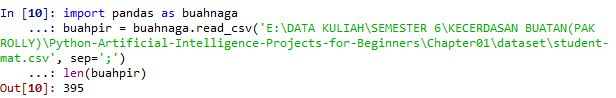
\includegraphics[width=1\textwidth]{figures/huda/1_hari4.JPG}}
		\caption{Hasil Codingan No 1.}
		\label{9}
\end{figure}
\item Penjelasan codingan ini berfungsi untuk menampilkan  baris  G1, G2 dan G3 ( berdasarkan kriterianya ) untuk kolom PASS pada variabel buahpir. Untuk lebih jelasnya, pada codingan terdapat pendefinisian pembacaan lamda ( panjang gelombang ) dari baris G1, G2 dan G3. Apabila row-row tersebut bernilai lebih dari 35 maka akan terdefinisikan angka 1 apabila tidak, maka akan terdefinisikan angka 0 pada kolom PASS ( sesuai permintaan awal ). Selanjutnya variabelnya di ditampilkan sehingga menampilkan keluaran. Tidak lupa terdapat juga jumlah dari baris dan kolom yang terubah sesuai dengan baris yang dieksekusi.
\subitem Gambar Screenshootan codingan dan hasil bisa dilihat pada gambar \ref{10}.
\begin{figure}[ht]
		\centerline{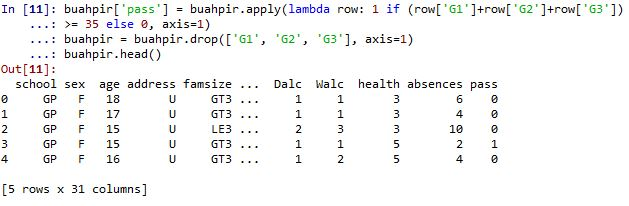
\includegraphics[width=1\textwidth]{figures/huda/2_hari4.JPG}}
		\caption{Hasil Codingan No 2.}
		\label{10}
\end{figure}
\item Penjelasan codingan ini mendefinisikan pemanggilan get dummies dari buahnaga dalam variabel buahpir. Di dalam get dummies sendiri akan terdefinisikan variabel buahpir dengan kolom-kolom yang akan dieksekusi seperti school, address dll. Kemudian variabel tersebut diartikan untuk mendapatkan kembalian berupa keluaran dari eksekusi perintah variabel buahpir beserta dengan jumlah baris dan kolom data yang dieksekusi.
\subitem Gambar Screenshootan codingan dan hasil bisa dilihat pada gambar \ref{11}.
\begin{figure}[ht]
		\centerline{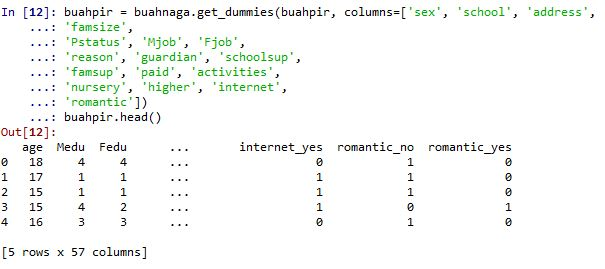
\includegraphics[width=1\textwidth]{figures/huda/3_hari4.JPG}}
		\caption{Hasil Codingan No 3.}
		\label{11}
\end{figure}
\item Penjelasan codingan ini difungsikan untuk mengartikan pembagian data yang berupa training dan testing data. pertama-tama variabel buahpir akan mengartikan sampel yang akan digunakan ( berupa shuffle row ) . Nah kemudian masing-masing parameter yaitu buahpir train dan buahpir test akan berjumlah 500 data ( telah dibagi untuk training dan testing ). Selanjutnya dilakukan pengeksekusian untuk kolom Pass, apabila sesuai dengan axis=1 maka eksekusi fungsi berhasil. Selain itu juga disertakan jumlah dari peserta yang lolos dari semua nilai data setnya.  
\subitem Gambar Screenshootan codingan dan hasil bisa dilihat pada gambar \ref{12}.
\begin{figure}[ht]
		\centerline{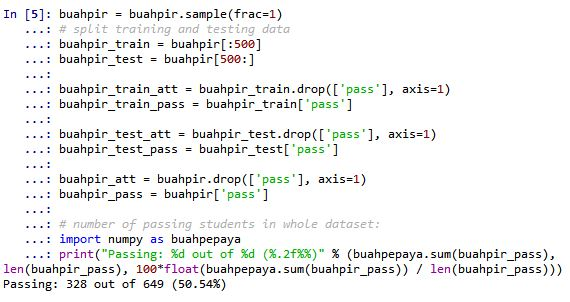
\includegraphics[width=1\textwidth]{figures/huda/4_hari4.JPG}}
		\caption{Hasil Codingan No 4.}
		\label{12}
\end{figure}
\item Penjelasan codingan ini hanya membuktikan pengujian dari Klasifikasi Decision Tree yang ada, apakah true atau tidak dan hasilnya true. Pada codingan ini di definisikan library sklearn untuk mengimpot atau menampilkan tree. Variabel buahapel difungsikan untuk membaca klasifikasi decision tree dari tree itu sendiri dengan 2 parameternya yaitu kriteria=entropy dan max depth=5. Maka selanjutnya variabel buahapel akan masuk dan terbaca dalam module fit dengan 2 parameter yaitu buahpir trai att dan buahpir train pass.
\subitem Gambar Screenshootan codingan dan hasil bisa dilihat pada gambar \ref{13}.
\begin{figure}[ht]
		\centerline{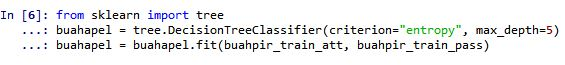
\includegraphics[width=1\textwidth]{figures/huda/5_hari4.JPG}}
		\caption{Hasil Codingan No 5.}
		\label{13}
\end{figure}
\item Penjelasan codingan ini memberikan gambaran dari klasifikasi decision tree yaitu pengolahan parameter yang dieksekusi kedalam variabel buahapel. Tentunya dengan pemanfaatan library graphviz yang telah diimport dan difungsikan.
\subitem Gambar Screenshootan codingan dan hasil bisa dilihat pada gambar \ref{14}.
\begin{figure}[ht]
		\centerline{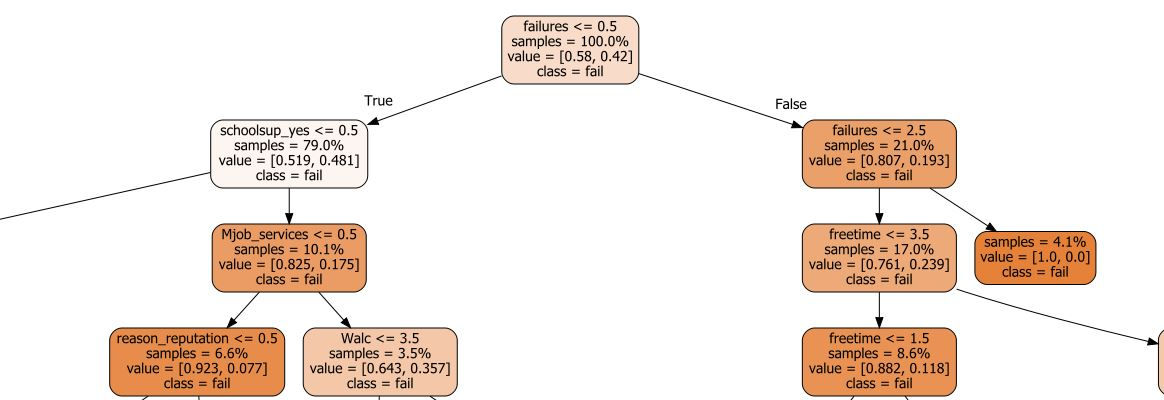
\includegraphics[width=1\textwidth]{figures/huda/6_hari4.JPG}}
		\caption{Hasil Codingan No 6.}
		\label{14}
\end{figure}
\item Penjelasan codingan ini membahas tentang penyimpanan tree dari library graphviz yang dieksekusi bersamaan dengan variabel buahapel dan parameter lainnya. Dilakukan pengecekan dan pengujian apakah klasifikasi decision treenya dapat berjalan atau tidak. Apabila tidak berjalan, maka akan terjadi error, namun codingan ini berfungsi.
\subitem Gambar Screenshootan codingan dan hasil bisa dilihat pada gambar \ref{15}.
\begin{figure}[ht]
		\centerline{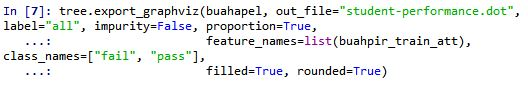
\includegraphics[width=1\textwidth]{figures/huda/7_hari4.JPG}}
		\caption{Hasil Codingan No 7.}
		\label{15}
\end{figure}
\item Penjelasan codingan ini membaca score dari variabel buahapel dimana terdapat 2 parameter yang dihitung dan diuji yaitu buahpir test att dan buahpir test pass. Untuk hasilnya sendiri mengapa berupa angka, dikarenakan pada parameter yang dieksekusi memang memiliki data sehingga dieksekusi dan menghasilkan keluaran dari score tersebut.
\subitem Gambar Screenshootan codingan dan hasil bisa dilihat pada gambar \ref{16}.
\begin{figure}[ht]
		\centerline{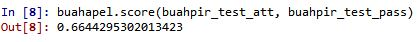
\includegraphics[width=1\textwidth]{figures/huda/8_hari4.JPG}}
		\caption{Hasil Codingan No 8.}
		\label{16}
\end{figure}
\item Penjelasan codingan ini membahas mengenai pengkesekusian fungsi dan variabel dari library yang didefinisikan dan yang diimport. Penjelasan lebih jelasnya ialah codingan ini mendefinisikan library sklearn.model.selection kemudian mengimport cross val score. Kemudian variabel score mendefinisikan cross val score yang telah diimport tadi dengan 4 parameter yaitu buahapel, buahpir att, buahpir pass dan cv=5 untuk dieksekusi. Setelah semua pemrosesan tersebut maka hasil yang di tampilkan ialah rata2 perhitungan dari variabel score dimana dan standar dari plus minusnya tentunya dengan ketentuan parameter Accuracy .
\subitem Gambar Screenshootan codingan dan hasil bisa dilihat pada gambar \ref{17}.
\begin{figure}[ht]
		\centerline{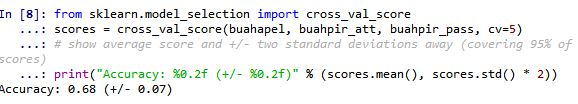
\includegraphics[width=1\textwidth]{figures/huda/9_hari4.JPG}}
		\caption{Hasil Codingan No 9.}
		\label{17}
\end{figure}
\item Penjelasan Codingan ini mendefinisikan max depth dalam jarak angka antara parameter 1 dan 20. Variabel buahapel mendefinisikan klasifikasi decision tree dengan 2 parameter. Kemudian variabel score mengeksekusi parameter lainnya yaitu seperti buahapel, buahpir att, buahpir pass dan cv=5 ) . Hasil yang ditampilkan ialah dari max depth, accuracy dan plus minusnya dan akhirnya hasil outputannya keluar.
\subitem Gambar Screenshootan codingan dan hasil bisa dilihat pada gambar \ref{18}.
\begin{figure}[ht]
		\centerline{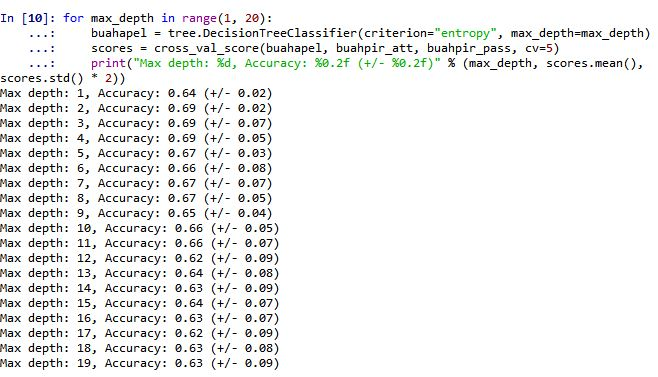
\includegraphics[width=1\textwidth]{figures/huda/10_hari4.JPG}}
		\caption{Hasil Codingan No 10.}
		\label{18}
\end{figure}
\item Penjelasan codingan ini mengartikan bahwa variabel depth\_acc akan mengeksekusi empty dari importan library numphy yang dinamakan buahpepaya dengan 2 parameter yaitu 19,3 dan float. i didefinisikan dengan angka 0 kemudian untuk perhitungan jarak max depth diantara parameter 1 dan 20. Variabel buahapel mengartikan klasifikasi decision tree dengan 2 parameter. setelah itu, variabel score mendefinisikan variabel depth\_acc dengan i dan 0, variabel kedua dari depth\_acc dengan i dan 1 serta variabel ketiga dari depth\_acc dengan i dan 2, maka pengeksekusian akhir bahwa variabel i akan ditambah dengan angka 1 untuk hasil akhirnya. Keluarannya akan berupa array dari perhitungan parameter dan variabel yang telah didefinisikan sebelumnya.
\subitem Gambar Screenshootan codingan dan hasil bisa dilihat pada gambar \ref{19}.
\begin{figure}[ht]
		\centerline{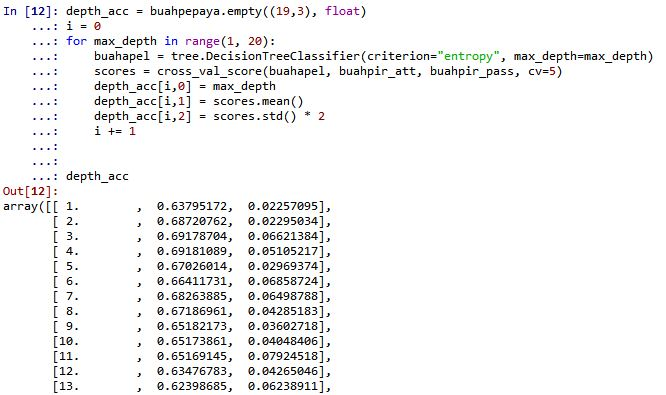
\includegraphics[width=1\textwidth]{figures/huda/11_hari4.JPG}}
		\caption{Hasil Codingan No 11.}
		\label{19}
\end{figure}
\item Penjelasan codingan ini mendefinisikan pemanggilan dari library matplotlib.pyplot sebagai buahanggur sehingga nanti hasilnya akan berbentuk gambar grafik/gelombang. Untuk variabel fig dan ax akan mendefinisikan subplots dari buahanggur. Setelah itu ketentuan dari parameter depth acc = 0, depth acc = 1 dan depth acc 2. Selanjutnya untuk menampilkan gelombang maka panggil variabel buahanggur dengan perintah show.
\subitem Gambar Screenshootan codingan dan hasil bisa dilihat pada gambar \ref{20}.
\begin{figure}[ht]
		\centerline{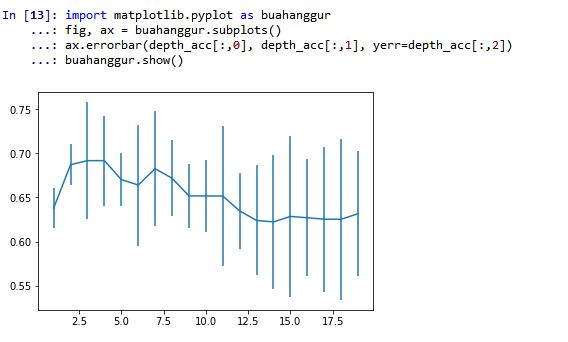
\includegraphics[width=1\textwidth]{figures/huda/12_hari4.JPG}}
		\caption{Hasil Codingan No 12.}
		\label{20}
\end{figure}
\end{enumerate}

\subsection{Penanganan Eror}
\begin{enumerate}
\item ScreeShootan Eror pada codingan No 8 dapat dilihat pada gambar \ref{21}.
\subitem 
\begin{figure}[ht]
		\centerline{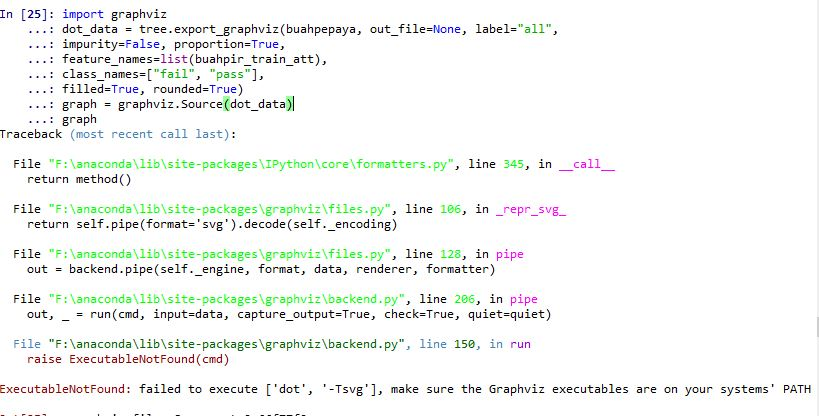
\includegraphics[width=1\textwidth]{figures/huda/eror6.JPG}}
		\caption{Hasil Gambar Eror No 6.}
		\label{21}
\end{figure}
\item Codingan eror dan jenis erornya : sebenarnya tidak terdapat eror pada codingan ini namun saat pertama kali di run current cell codingan ini akan eror dan tidak keluar outputannya dikarenakan library graphviz sebelumnya tidak ditemukan atau belum di install terlebih dahulu.
\subitem 
\begin{verbatim}
import graphviz
dot_data = tree.export_graphviz(buahapel, out_file=None, label="all", impurity=False, proportion=True,
                                feature_names=list(buahpir_train_att), class_names=["fail", "pass"], 
                                filled=True, rounded=True)
graph = graphviz.Source(dot_data)
graph
\end{verbatim}
\item Solusi pemecahan masalah eror tersebut yaitu dengan cara menginstall terlebih dahulu library graphviznya pada anaconda prompt atau command prompt anda dengan perintah conda install graphviz setelah itu run kembali codingan No 8 maka akan muncul outputan atau tampilan keluarannya.
\subitem Berikut gambar cara menginstall graphviz dapat dilihat pada gambar \ref{22}
\begin{figure}[ht]
		\centerline{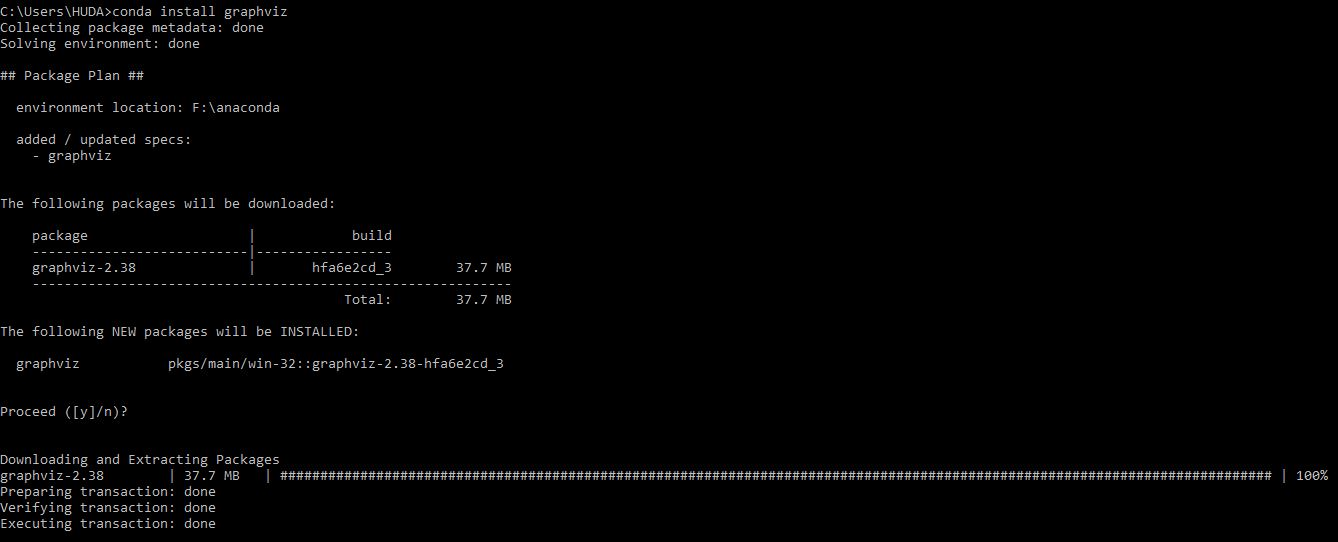
\includegraphics[width=1\textwidth]{figures/huda/penangananeror6.JPG}}
		\caption{Hasil Gambar Penanganan Eror No 6.}
		\label{22}
\end{figure}
\end{enumerate}


\begin{figure}[ht]
		\centerline{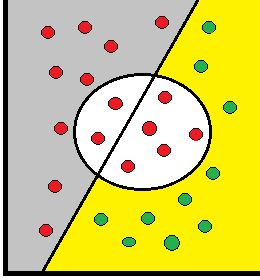
\includegraphics[width=1\textwidth]{figures/huda/binary.JPG}}
		\caption{Binary Classification.}
		\label{1}
\end{figure}
\begin{figure}[ht]
		\centerline{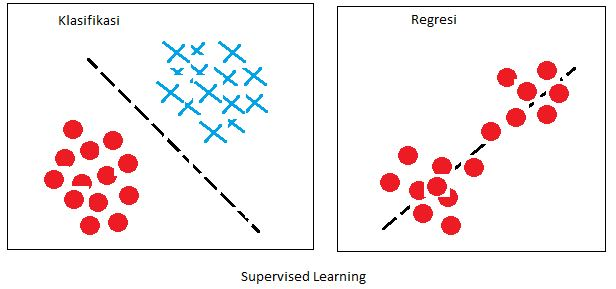
\includegraphics[width=1\textwidth]{figures/huda/supervised.JPG}}
		\caption{Supervised Learning.}
		\label{2}
\end{figure}
\begin{figure}[ht]
		\centerline{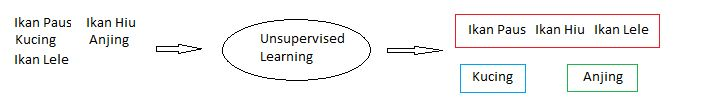
\includegraphics[width=1\textwidth]{figures/huda/unsupervised.JPG}}
		\caption{Unsupervised Learning.}
		\label{3}
\end{figure}

\begin{figure}[ht]
		\centerline{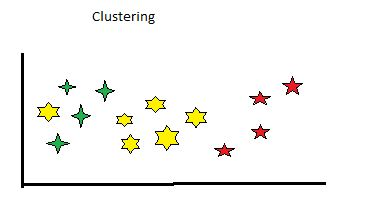
\includegraphics[width=1\textwidth]{figures/huda/clustering.JPG}}
		\caption{Clustering.}
		\label{4}
\end{figure}
\begin{figure}[ht]
		\centerline{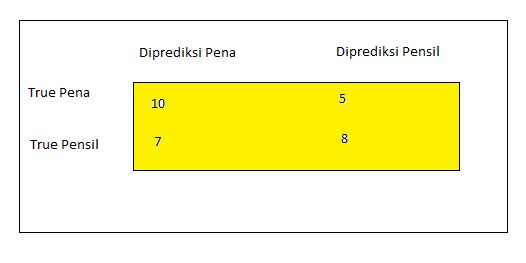
\includegraphics[width=1\textwidth]{figures/huda/evaluasidanakurasi.JPG}}
		\caption{Evaluasi dan Akurasi.}
		\label{5}
\end{figure}
\begin{figure}[ht]
		\centerline{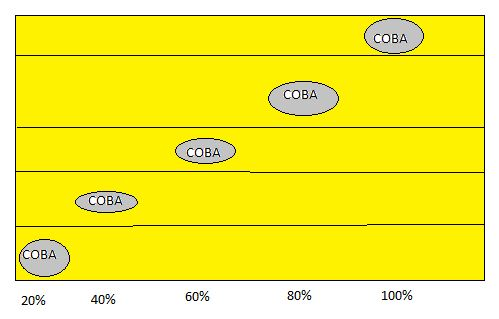
\includegraphics[width=1\textwidth]{figures/huda/K-fold.JPG}}
		\caption{K-fold Cross Validation.}
		\label{6}
\end{figure}
\begin{figure}[ht]
		\centerline{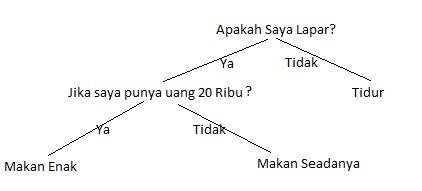
\includegraphics[width=1\textwidth]{figures/huda/DecisionTree.JPG}}
		\caption{Decision Tree.}
		\label{7}
\end{figure}
\begin{figure}[ht]
		\centerline{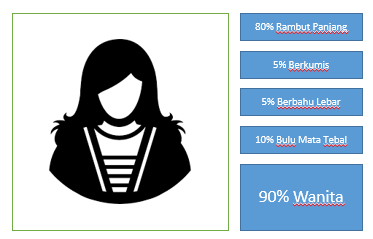
\includegraphics[width=1\textwidth]{figures/huda/Gain.PNG}}
		\caption{Gain.}
		\label{8}
\end{figure}

